% Euclidean Handout Number Two 
\documentclass{tufte-handout}

%\geometry{showframe}% for debugging purposes -- displays the margins

%%%% Packages to make things pretty
\usepackage{amsmath,amsthm}
\usepackage{booktabs}
\usepackage{graphicx}
\setkeys{Gin}{width=\linewidth,totalheight=\textheight,keepaspectratio}
\graphicspath{{graphics/}}
\usepackage{units}
\usepackage{fancyvrb}
\fvset{fontsize=\normalsize}
\usepackage{multicol}
\usepackage{pdfpages}

%%%% Theorem Evironments
\theoremstyle{definition}
\swapnumbers
\newtheorem{problem}{Problem}[section]
\newtheorem{conjecture}[problem]{Conjecture}
\newtheorem*{definition}{Definition}
\newtheorem*{theorem}{Theorem}
\newtheorem{question}[problem]{Question}
\newtheorem{challenge}[problem]{Challenge}
\newtheorem*{postulate}{Postulate}

%%%%%

\title{Euclidean Geometry:\\An Introduction to Mathematical Work}
\author[]{Math 3600}
\date{Fall 2016}

\begin{document}

\maketitle

\begin{marginfigure}
    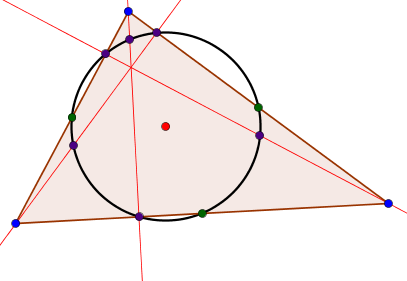
\includegraphics{NPC}
\end{marginfigure}

\vspace{.5in}
Here are some experimental problems I have never reached with this course.

\setcounter{section}{19}
\section{The Simpson Line}

\begin{problem}\label{prob:Simson-line}
Let $ABC$ be a triangle. Let $P$ be a point on the circumscribed circle of $ABC$. Let $D, E, F$ be the feet of the perpendiculars from $P$ to the sides of the triangle (possibly extended). Show $D, E$ and $F$ are collinear.
\end{problem}

\begin{definition}\label{defn:Simson-line}
The line just found is called the \emph{Simson line} of $P$ with respect to $ABC$.
\end{definition}


\section{Some Basic Projective Geometry}

\begin{problem}[Menelaus' Theorem]\label{prob:Menelaus-theorem}
Let $ABC$ be a triangle. Let a line $\ell$ cut the (extended) sides of $ABC$ at $D, E, F$. Then
\[ AD\cdot BF \cdot CE = BD \cdot CF \cdot AE .\]
\end{problem}


\begin{center}
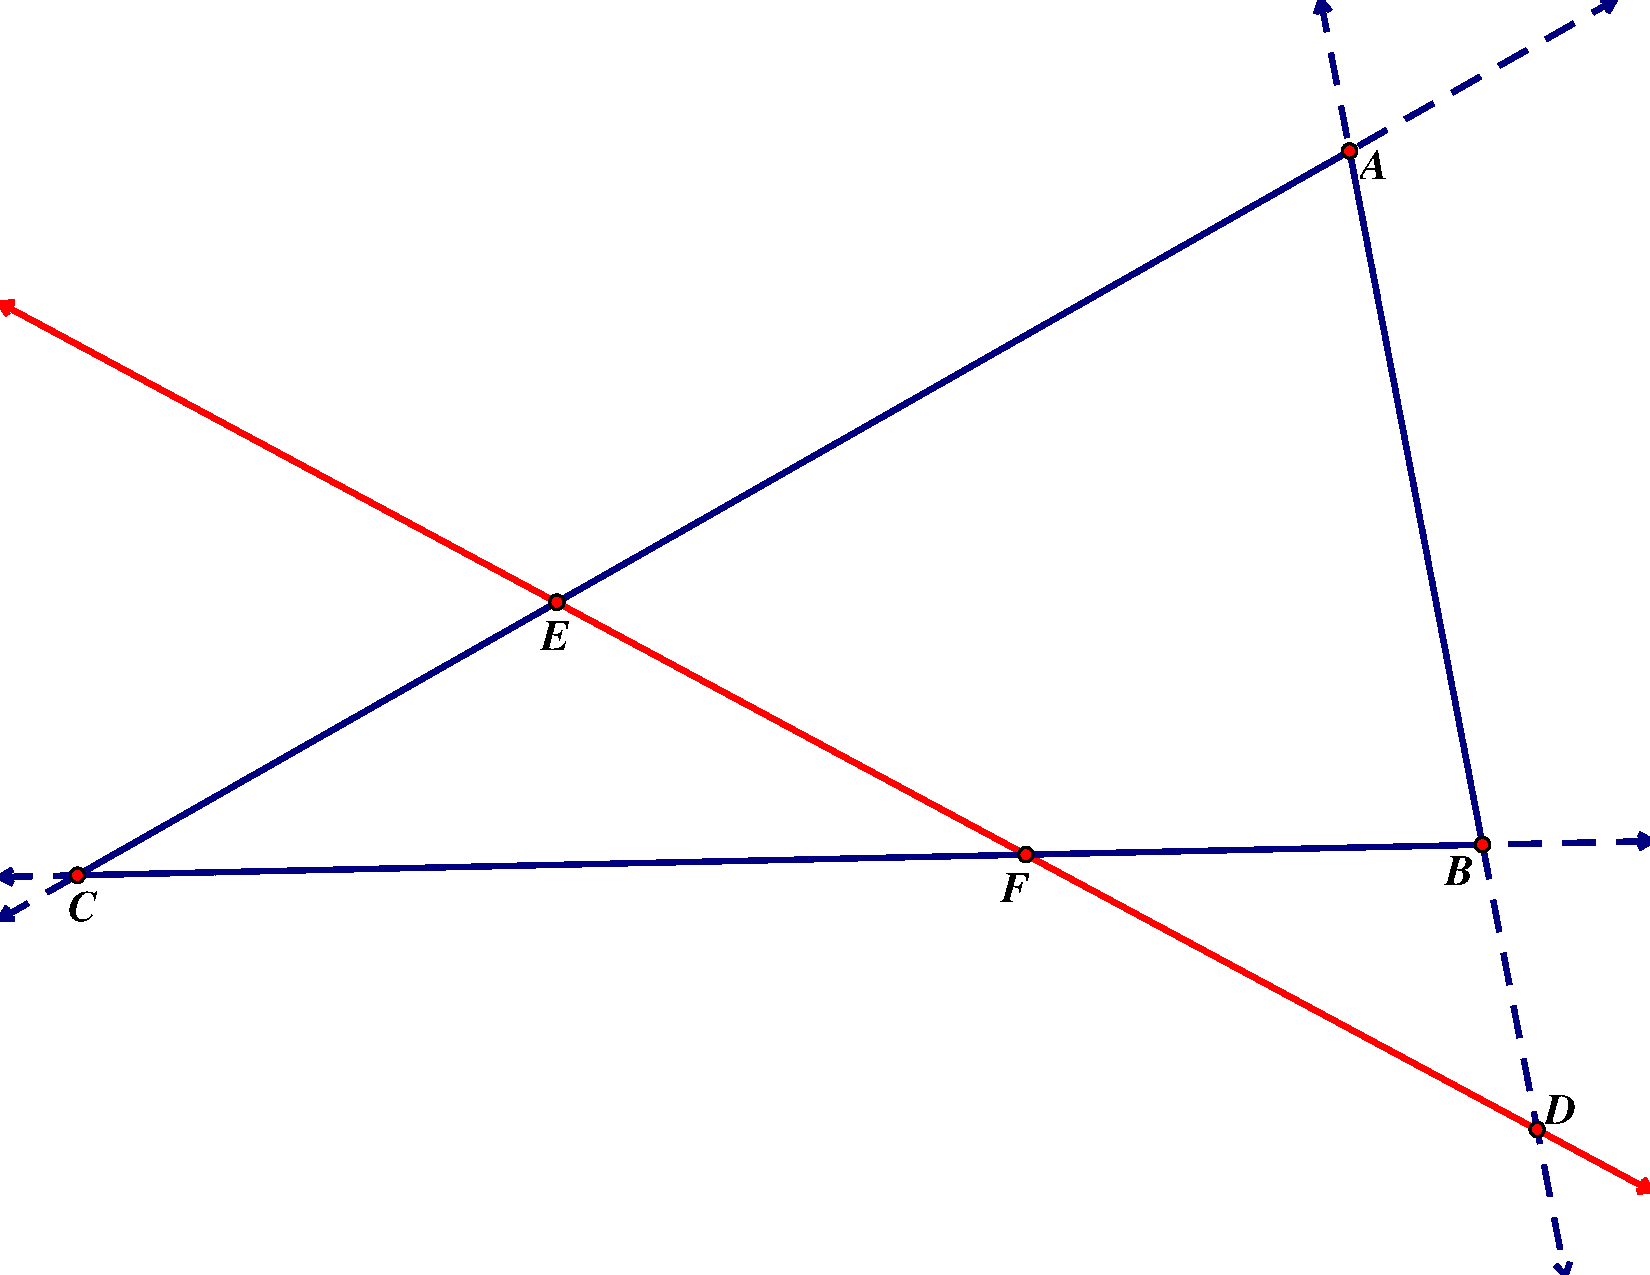
\includegraphics[width=.9\textwidth]{Menelaus.pdf}
\end{center}

\begin{problem}
Show the converse is also true!
\end{problem}

\noindent\textbf{Note:} This result is usually stated
\[ 
\dfrac{AD}{DB}\dfrac{BF}{FC}\dfrac{CE}{EA} = -1
\]
and the segments are interpreted as \emph{signed} segments, where the direction of travel matters!

\begin{problem}[Ceva's Theorem] \label{prob:Ceva-theorem}
Let $ABC$ be a triangle, and let $P$ be any point inside the triangle. Draw lines from the vertices through $P$ meeting the opposite sides at $D, E, F$. Show that 
\[ AD\cdot BF\cdot CE = BD \cdot CF \cdot AE \]
\end{problem}

\begin{center}
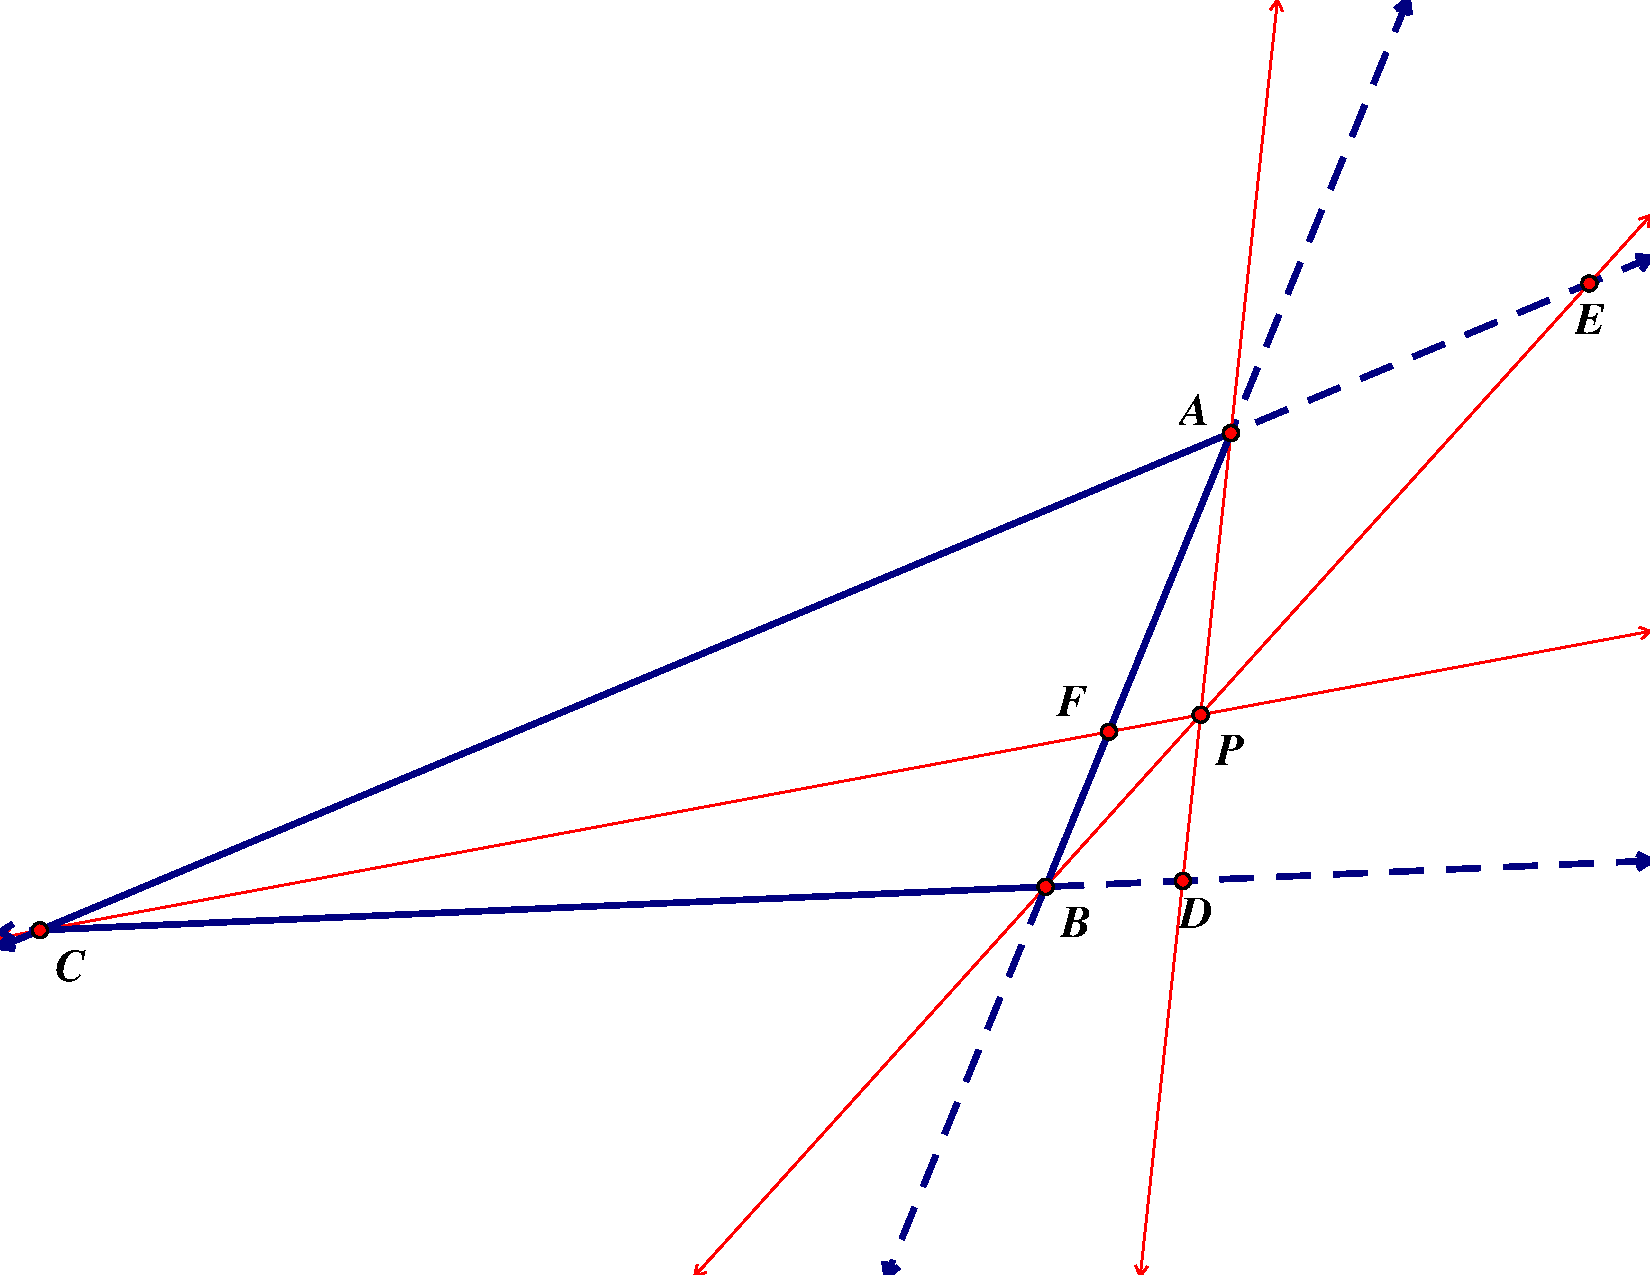
\includegraphics[width=.9\textwidth]{Ceva.pdf}
\end{center}

\begin{problem}
Show the converse!
\end{problem}

Note, this also has a more standard restatement. What should it be?


\begin{problem}[Desargues' Theorem]\label{prob:Desargue's-special-case}
Let $ABC$ and $A'B'C'$ be two triangles. Suppose that the lines $AA'$, $BB'$ and $CC'$ are concurrent at a point $O$. Suppose that $AB$ is parallel to $A'B'$ and $BC$ is parallel to $B'C'$. Show that $AC$ is parallel to $A'C'$.
\end{problem}



\vfill
\end{document}
